\documentclass{acm_proc_article-sp}
\usepackage{url}
\usepackage{graphicx}
% \usepackage[algosection, vlined, linesnumbered]{algorithm2e}
\usepackage{algorithm}
\usepackage{algpseudocode}
\usepackage{enumitem}
\usepackage{subfigure}
\usepackage{colortbl}
\usepackage[table,xcdraw]{xcolor}

\pagenumbering{arabic}

\begin{document}
\sloppy

\title{Dataset Ranking using Citation and Coauthorship Networks}

\numberofauthors{4} %  in this sample file, there are a *total*
% of EIGHT authors. SIX appear on the 'first-page' (for formatting
% reasons) and the remaining two appear in the \additionalauthors section.
%
\author{
% 1st. author
\alignauthor
Hannah Chen\\
       \affaddr{Computer Science and Engineering}\\
       \affaddr{University of CA, San Diego} \\
       \email{hechen@eng.ucsd.edu}
% 2nd. author
\alignauthor
Xiaoqian Jiang\\
       \affaddr{Department of Biomedical Informatics}\\
       \affaddr{University of CA, San Diego}\\
       \email{x1jiang@ucsd.edu}
% 3rd. author
\alignauthor 
Arya Iranmehr\\
       \affaddr{Electrical and Computer Engineering} \\
       \affaddr{University of CA, San Diego}\\
       \email{airanmehr@ucsd.edu}
% \and  % use '\and' if you need 'another row' of author names
% 4th. author
\and
\alignauthor 
Shuang Wang\\
       \affaddr{Department of Biomedical Informatics}\\
       \affaddr{University of CA, San Diego}\\
       \email{wsasyz@gmail.com}
}

\maketitle

\begin{abstract}
Biomedical sciences is increasingly moving towards data driven approaches. Unfortunately, the vast majority of biomedical datasets are underutilized after their initial publications due to the increased rate of dataset generation and difficulty in searching for relevant datasets. Efficient use of these existing datasets requires identifying important datasets for a given researcher to explore, which may be based on a combination of an individual's research interests, past publications and authorship network. 

Bibliometrics and citation analysis have been used to find features, impact, and interrelationships between researchers and papers as well as to establish precedence of ideas and results offering evidence of the quality and significance of scientific work. Drawing insights from PageRank, three ranking approaches are implemented on a heterogeneous biomedical information network connected to nine breast cancer data series found in the Gene Expression Omnibus (GEO) data repository. 

Author ranking results are qualitatively compared to show that the Multirank approach best fits the needs of the DataRank project, a personalized online recommendation system for biomedical datasets. Using the results of author and journal Multiranking, conditional probabilities of datasets given author are calculated. This enhances the DataRank system by adding citation analysis to its existing methods of generating features used to rank dataset recommendations.
\end{abstract}


\section{Introduction}
New advancements in technologies have resulted in the proliferation of data production at an unprecendented scale, leading scientists to the problem that the capacity to organize, let alone find or understand the data, has lagged behind our ability to generate data. Back in 2006, shortly after the popularization of next-generation sequencing, it was found that data volumnes were doubling every year and becoming increasingly complex and correlated over many dimensions~\cite{szalay20062020}. Using nucleotide sequencing as an example, it was found in 2009 that submission rates to a global database were growing at 200\% per annum; conservation of this data is guarded by three global repositories which exchange new data on a daily basis~\cite{southan2009beyond}.

Alongside this proliferation, where invested financial resources may be provided by the public sector, follows an expectation of freely accessible data for global biomedical research. As such, much of the scientific community has been concerned with the scalability and collaborative issues associated with data management like necessary standardization and infrastructure needed to support useful processing and workflow methods. Increased commitments to data sharing is reinforced by efforts dedicated to building databases, repositories and biobanks~\cite{leonelli2012introduction}. Multidisciplinary databases also led to the collection and combined analysis of data found from multiple repositories, which eventually may be deposited elsewhere for shared use. In a generation of data-intensive and data-driven computing, scientists are engaging in records as a corpus of text and collections of interlinked data resources that may identify papers of interest, suggest hypotheses to explore, and even the production of new data~\cite{lynch2009jim}.

Existing entities have been addressing issues to facilitate data use: the European Bioinformatics Institute has developed open standards and search systems indexing data, and the National Center for Biotechnology Information (NCBI) has invested greatly in the PubMed~\cite{pubmed} search engine for accessing biomedical literature citations of the MEDLINE database. Despite these efforts, the growing size and number of partially coordinated and incompatible data set formats makes data discovery and integration a notable challenge. For example, author analysis on Pubmed is driven by crawling, so manually converting this into structured data before analysis is a task in and of itself. But before even considering the issues of mining these vast troves of data, one needs to somehow identify these relevant data sets.

This paper proposes a way to augment the recommendation framework currently utilized in the DataRank~\cite{datarank} prototype which aims to rank datasets based on generated features and users' feedback. By exploring several ranking approaches on citation and authorship networks, publications and authors can be individually or synchronously ranked with their ranking values represented as a probability distribution. Datasets are associated with papers as a linear combination of weights, and a ranking metric is used to generate conditional probabilities for datasets given author.

\section{Background}
In the past, people may have cited dataset identification numbers explicitly, cited the publication connecting to the dataset's first use, merely mentioned it within a paper, or not cited the dataset at all. Authors and publishers are now encouraged to include data availability information in publications. While much work has focused on PubMed article querying, there still lacks of a unified, systematic way to retrieve datasets.

In 2012, the National Institute of Health launched the Big Data to Knowledge (BD2K) initiative with one of its goals to address poor data accessibility through development of a ``set of platforms and tools by which biomedical researchers can find, reanalyze, and reuse data and which will support data citation metrics and precise scholarly attribution for data''~\cite{bd2k}. One project in particular, bioCADDIE, is developing a Data Discovery Index prototype that aims to have a free, user-friendly means for users to locate data sets of interest. In the long-term, bioCADDIE hopes to be as transformative and impactful for data as PubMed for the biomedical literature~\cite{biocaddie}. The many different use cases and dataset origins proves to be a complication for dataset indexing. For example, a repository may have strict guidelines to only accept primary datasets, not reanalysis, metaanalysis or comparisons. Datasets may also be collected over a range of time, published at various times, or be a subset or derivative of larger, dynamic databases.

To emphasize the current difficulty in searching for datasets, we ask: What is the existing way to search? A direct search requiring background knowledge on the part of the enquirer can be done by searching within a repository for the data or authors directly connected to the dataset. There are also experts who provide searchable lists of curated data sets. The National Institute of Health (NIH) currently manages 65 biomedical data sharing repositories. In the best case, NIH may have invested resources to provide user-friendly mechanisms for query and analysis, such as with GEO. GEO records can be accessed directly using an accession number or queries can be made to study-level or gene-level databases. Queries can be ``effectively performed by simply entering appropriate keywords and phrases into the search box. However, given the large volumes of data stored in these databases, it is often useful to perform more refined queries''~\cite{geoquery}. In other words, efficiently querying requires already knowing what a dataset encompasses.

Finding particular datasets can also be done via MEDLINE citations via the secondary source identifier (SI). Beginning in 2005, many data types discussed within MEDLINE articles, such as sequencing data, gene expression data, and clinical trial data, could be included in the SI element. GEO accession numbers for data started in February 2006; 25 of 38 MEDLINE databank names had 2014 approximate start date to be included in SI field. Fortunately, this means that some dataset indexing can be queried through the NCBI/Entrez databse suite instead of matching regular expression rules, which was done for the DataRank prototype.

The issues with developing a biomedical dataset search engine is similar to what Google faced back in 1998: there is a rapidly growing amount of data leading to a diminishing return effect where retrieval becomes harder as the number and category of datasets increase, the number of users inexperienced in searching for relevant data sets increases, and the mental resources to parse through search results decrease. All this hints for the need of higher precision when targeting or personalizing results as the search space grows. Citation analysis and bibliometrics establish precedence of ideas and hint at the quality or significance of a scientific work. We apply these ideas to learn about datasets with the end goal of developing a personalized biomedical dataset search engine. 

The networks arising from PubMed/MEDLINE citations are inherently hetergeneous: multiple objects types have interactions with other types based on different relations. For example, researchers may cite others via journal publications, papers may belong to different topical areas, datasets may be shared and reanalyzed for different papers, and authors may be socially connected by collaboration, citation, or organizations. Figure~\ref{fig:hetero} shows an example of the object types and relations we explore with PubMed.

\begin{figure}[h]
    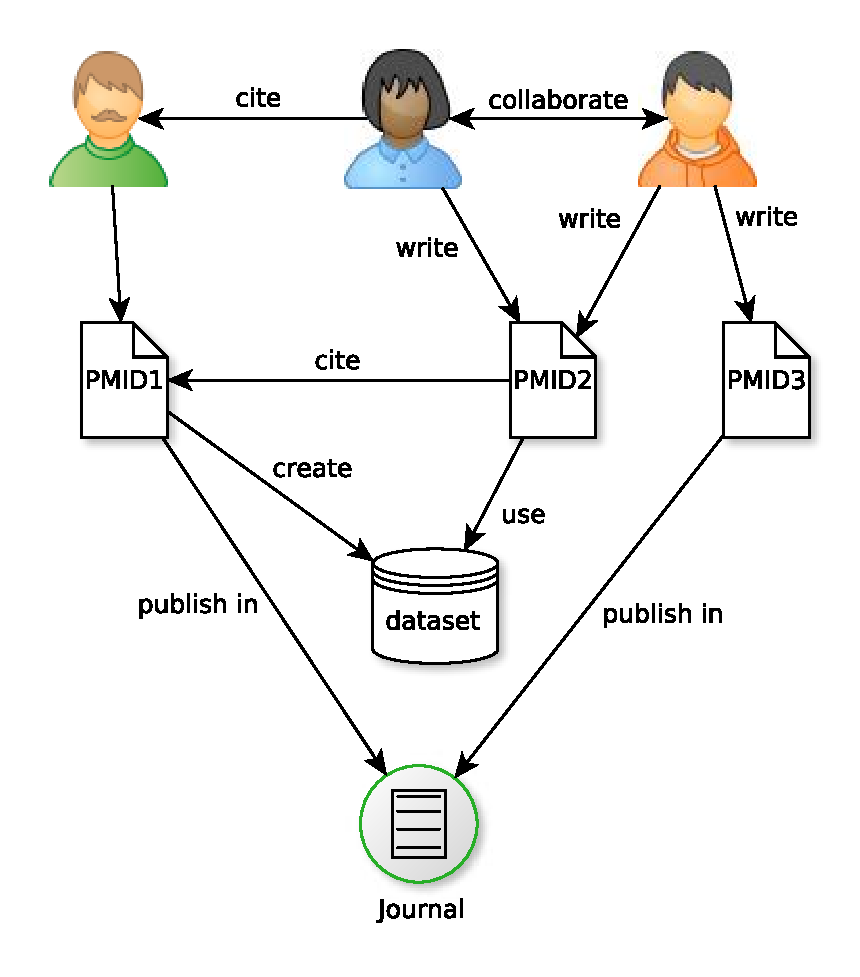
\includegraphics[width=\columnwidth]{hetero.eps}
    \caption{Small Heterogeneous Network}
    \label{fig:hetero}
\end{figure}

\section{Related Work}
\label{sec:related}
Many statistical averages or indices have been proposed in bibliometrics as a measurement of bibliographic importance, such as impact factor (average citations received during two preceding years)~\cite{garfield1972citation}, immediacy index (number of citations received in a given time frame divided by the number of articles published for journal), cited half-life (median age of cited articles)~\cite{elsevier}, and Hirsch index (based on some of citation distribution)~\cite{hirsch2005index}. Centrality measures, which identify important vertices within networks, have also been used for ranking, typically in a social network environment. The four most common of these measures include degree centrality (degree number of the node), betweenness centrality (number of shortest paths that pass through the node), closeness centrality (reciprical of the sum of a node's shortest path from all other nodes), and eigenvector centrality.

Prioritization of relevant datasets added to the immense scale of the biomedical search space share similar problems to search engines and webpage ranking. It's thus no surprise that a large amount of work in bibliometrics and ranking has borrowed ideas from web ranking, specifically PageRank~\cite{pagerank} and HITS~\cite{hits}. PageRank makes use of the web's hyperlink structure to give an approximation of a web page's importance or quality. It is stated as an eigenvalue problem of solving for a stationary probability distribution that is described by a random walk on the graph of a web network. The pagerank metric constitutes the probability of a random surfer (a web surfer who is given pages at random and keeps clicking links, eventually getting bored and starting on another random page) arriving at a page. The HITS algorithm follows a mutual reinforcement principle by using two scores to rank webpages: an authority score estimates the value of the pages's content and a hub score measures the value of the pages's links to other pages. These works all feature recommendation based on ranking designed for a homogeneous system, with web pages as the single object type and links between pages as the relation or edges of the network. 

Building upon these and applying the methods to heterogeneous networks, PopRank~\cite{nie2005object} adds popularity to each link in the PageRank framework, Deng et al.~\cite{deng2009generalized} explore a generalized co-HITS algorithm to incorporate a bipartite graph with content information from both sides of the graph, and~\cite{zhu2007combining} combines content and links for hypertext classification through matrix factorization.

Moving towards the multi-dimensional space, tensors have been utilized to represent multi-relational data with much work on efficient mathematical frameworks and algorithms in tensor factorization to solve a set of multivariate polynomial equations arising from these data. For example, MetaFac~\cite{lin2009metafac} proposes a hypergraph representation and its factorization to discover community structure in rich networks, TOPHITS~\cite{kolda2006tophits} adds anchor text of links to the computation of hub and authority scores through tensor rank decomposition, and cubeSVD~\cite{sun2005cubesvd} incorporates user clickthrough data to personalize web search with the use of high-order singular value decomposition techniques. 


    \begin{table}[h]
    \centering
    \resizebox{\columnwidth}{!}{
    \begin{tabular}{|c|c|c|}
    \hline
    \textbf{\begin{tabular}[c]{@{}c@{}}Feature / \\ Network Property\end{tabular}} & \textbf{Data} & \textbf{Metadata} \\ \hline
    \textbf{Homogeneous} & --- & \begin{tabular}[c]{@{}c@{}}Impact Factor, immediacy index;\\ PageRank, HITs\end{tabular} \\ \hline
    \textbf{Heterogeneous} & OmicSeq & \begin{tabular}[c]{@{}c@{}}Corank, Multirank, PopRank, co-HITS; \\ MetaFac, TOPHITS, cubeSVD;\\ RankClus, NetClus\end{tabular} \\ \hline
    \end{tabular}}
    \caption{Summary of Related Work based on Feature vs. Network Property}
    \label{tab:related}
    \end{table}


In addition to using ranking measures to make recommendations, clustering approaches have been used for recommendation systems by identifying similar objects via grouping and propagating information from these similar objects. RankClus~\cite{sun2009rankclus} integrates clustering with ranking on hetergeneous information networks. NetClus~\cite{varadharajalu2011author} builds upon this by adding an author disambiguation technique and applies it to PubMed data.

Finally, the most comparable prototype is the biomedical knowledge discovery system OmicSeq~\cite{omicseq} (currently in beta) led by Dr. Zhaohui Steve Qin, who incidentally has been brought on as a collaborator of the bioCADDIE umbrella. OmicSeq gives researchers easy access to data by building a database emcompassing publicly available omics data and providing a ranked data browser to efficiently browse and gain insights through hidden functional relationships. His browser allows direct gene querying, rather than querying with metadata. OmicSeq uses their ``trackRank algorithm''. This two-step ranking first ranks the percentage of each gene's expression within a dataset compared to all other gene expressions in the dataset, then ranks these rankings between datasets.
% which is based on the idea that a gene plays an important role in a dataset if its score ranks at the top among all genes in the genome, to rank results. 


\paragraph{DataRank}
Our results of author and journal rankings is used to calculate conditional rankings between authors and datasets to enhance the DataRank~\cite{datarank} project. DataRank aims to make personalized data recommendations based on content similarity and user background. Here a quick summary of the existing prototype is discussed.

First, a bipartite citation graph between datasets and publications is created by crawling PMC dataset citations using regular expressions based on dataset naming rules. Then dataset features are generated as a binary vector of MeSH terms propogated from the MeSH terms of its citing publications. Finally, datasets are ranked based on a combination of these generated features and user feedback. 

Ranking follows a Bayesian approach and occurs in two phases: offline mode and online mode. The offline ranking given a query is the posterior distribution of dataset labels given evidence (query, dataset prior, and dataset features). This is found to be proportional to query likelihood and dataset prior, which they have defined as a Tanimoto coefficient and number of citations, respectively. The online algorithm takes user rating feedback to calculate another posterior distribution to present user-specific dataset rankings. Here the prior is simply the posterior calculated during the offline phase, and the likelihood is a normalization of estimated unknown user ratings. This estimate is a weighted linear combination of all rated datasets where weights are proportional to similarity (Jaccard index) between items.

While an encouraging prototype, there are a number of limitations. The naive collaborative filtering model only takes into consideration dataset features using MeSH terms and ignores any user features. The system also ignores any temporal dependencies: search sessions are independent and rating results are not transferable. Lastly, any network influences contained in the citation network are not captured, and the dataset/publication authorship network, which may also provide some user-level features, is omitted. (Presumably, the users of this product may be researchers themselves within this author network.)

This lack of user features and authorship network influence, in particular, is a key area of improvement in order to provide personalizable ranking results. Similarity measures between authors could be defined, and existing ratings of similar authors could be propagated to those users with fewer ratings. By conditioning on certain authors and user ratings, dataset rankings may be vastly different. Given particular datasets, we could also identify which authors are highly influential and perhaps incorporate this as features of the dataset.

\section{Ranking Frameworks}
By examining the state of the art methods from Section~\ref{sec:related} in the context of our problem and available data, we have identified two frameworks to explore. Corank~\cite{zhou2007co} and Multirank~\cite{ng2011multirank} are implemented to compare author rankings and resulted in three different ranking approaches: individual ranking, coranking, and multiranking. 

\subsection{Corank} 
Corank incorporates simple counting metrics, such as number of publications or number of citations, with network structure. It borrows ideas from previous ranking techniques, such as link analysis from PageRank and the mutual reinforcement principle of HITS, and applies this in the context of heterogeneous networks. Here it assumes a mutually reinforcing relationship between authors and publications: an author of higher rank will increase the rank of his or her publication, and a higher ranked publication will increase the rank of its authors. 

A symmetric collaboration network connects authors, a directed citation network connects papers, and a bipartite authorship network connects authors with papers. First, each network is ranked independently based on the PageRank paradigm by taking intra-class random walks on the author social network $G_A$ and the paper citation network $G_P$. We refer to this approch as `individual ranking' when executed independently of corank. These two are then coupled by an inter-class random walk by combining the author graph and citation graph with a bipartite authorship graph $G_{AP}$. The Corank approach is evaluated qualitatively by comparing it to other bibliometrics, like publication and coauthor count, and individual author ranking.


\paragraph{Intra-class Random Walks}
A stochastic process satisfies the Markov property if conditioned on the current state, the past state and future state are independent. We consider a random walk on a graph as a Markov chain and can define it as a transition probability matrix where each position $M_{i,j}$ is the conditional probability of jumping to vertex $j$ from the current vertex $i$. If there are no outgoing edges from vertex $i$ in the graph, let $M_{i,j} = \frac{1}{n}$ for all vertices $j$. The entries are nonnegative and every row adds to one. If it is possible to eventually get from every state (vertex) to every other state with some positive probability, it is termed an ergodic Markov chain. Each time step $t$ of the random walk results in a probability distribution vector by taking the dot product of the transition matrix \footnote{We take the transpose of the transition matrix to form a column stochastic matrix because it has an eigenvalue equal to one where the corresponding eigenvector is all postive.} with a probability distribution at time $t-1$, 
    \begin{equation}
        m_t = M^Tm_{t-1}.
    \end{equation}

The probability distribution vector $m$ can be interpreted as an individual ranking score for the vertices of a graph $G_M$ and can be repeatedly computed by a random walk on a transition matrix $M$. In order to guarantee that $M$ is ergodic, we manipulate it with a jump parameter $\alpha$, which denotes the probability of jumping to a vertex chosen uniformly at random instead of taking the random walk step
    \begin{equation}
        \tilde{M} = (1-\alpha)M + \frac{\alpha}{|m|} \textbf{1}\textbf{1}^T  
    \end{equation}
where $|m|$ is the number of vertices in graph $G_M$. $\alpha$ is similar to the dampening factor used in PageRank to encode the probability that a random surfer will become bored and go to another random page.

The stationary probability of an ergodic Markov chain can be obtained by solving $m = \tilde{M}m$ which involves taking powers of the transition matrix $\tilde{M}$ until $m$ is unchanged, or by solving for the left eigenvector of $\tilde{M}$ corresponding to the eigenvalue of 1 (part of the Perron Frobenius theorem for irreducible matrices). Each intra-class random walk begins with a matrix $M$ based on the graph $G_M$, and is then altered to create $\tilde{M}$ describing the random walk on the graph $G_M$. The intra-class walk occurs within the author network and the paper network. Below, we define matrices $A$ and $P$ formed from the author network and paper networks that are used to rank authors and papers, respectively.

The author social network is constructed by connecting two authors by a weighted edge if they collaborated on a paper. This is computed by first defining two authors' collaboration for a paper for authors $i,j$ and paper $p$:
    \begin{equation}
        \tau(i,j,p) = \frac{\mathbb{I}(i,j \in p)}{|p|(|p|+1)/2}    
    \end{equation}
where $|p|$ is the number of authors for paper $p$, and then summing the score over all papers to form the symmetric matrix:
    \begin{equation}
        T_{i,j} = \sum_{p \in P} \tau(i,j,p).
    \end{equation}

$T$ is normalized by rows to obtain the transition probability from author $a_i$ to author $a_j$:
    \begin{equation}
        Pr(j|i) = A_{i,j} = \frac{T_{i,j}}{\sum_j T_{i,j}}.
    \end{equation} 

The paper citation network is constructed by connecting two papers with a directed, unweighted edge from $p_i$ to $p_j$ if paper $i$ cites paper $j$. The transition probability from paper $p_i$ to paper $p_j$ is defined as 
    \begin{equation}
        Pr(j|i) = P_{i,j} = \frac{\mathbb{I}(i \rightarrow j)}{n_i},
    \end{equation}
where $n_i$ is the number of citations of paper $p_i$. A paper that does not cite any papers is given transition probability $\frac{1}{|P|}$.

As explained previously, the individual author ranking scores for vertices of $G_A$ are computed by solving the equation $a = \tilde{A}a$ and the individual paper ranking scores for vertices of $G_P$ are computed by solving the equation $p = \tilde{P}p$.


\paragraph{Inter-class Random Walk}
A heterogeneous graph is created by taking the union of the author graph, citation graph and a bipartite authorship graph. The bipartite authorship network is constructed by connecting an author to a paper he or she has published. It is represented as an adjacency matrix $E_{AP} \in \{0,1\}^{|A| \times |P|}$ where $E_{AP}(i,j) = 1$ indicates that paper $j$ is written by author $i$. The adjacency matrix is then weighted to form the matrix $W_{AP}$ where each $w(i,j)$ entry of the adjacency matrix is divided by the number of authors of the document $j$, or 
    \begin{equation}
        w(i,j) = \frac{E_{AP}(i,j)}{|n_j|} = \frac{\mathbb{I}(i \in n_j)}{|n_j|}
    \end{equation}

Two conditional probability matrices are formed from the weighted matrix when normalizing by either paper or author:
    \begin{equation}
        Pr(p_j|a_i) = AP_{i,j} = \frac{w(i,j)}{\sum_k w(i,k)}
    \end{equation}
where $AP \in \mathbb{R}^{|A|\times|P|}$ represents the probability of moving from author $i$ to paper $j$, and
    \begin{equation}
        Pr(a_i|p_j) = PA_{j,i} = \frac{w(i,j)}{\sum_kw(k,j)}    
    \end{equation}
where $PA \in \mathbb{R}^{|P|\times|A|}$ represents the probability of moving from paper $j$ to author $i$. 

The conditional probability matrices $AP$ and $PA$ describe the inter-class random walk that couples the author network and the citation network. An inter-class step jumps from author to paper or paper to author, and changes the probability distribution of $(\mathbf{a},\mathbf{p})$ to $(PA^T\mathbf{p},AP^T\mathbf{a})$. We let each inter-class jump take three substeps. For example an inter-class step from author to paper would involve $(\mathbf{a} \rightarrow \mathbf{p'} \rightarrow \mathbf{a'} \rightarrow \mathbf{p''})$\ and is outlined in Algorithm~\ref{alg:inter}.

    \begin{algorithm}
        \caption{Inter-walk procedure}
        \begin{algorithmic}[1]
        \Function{inter}{$U,V,x$}
            \State $y \leftarrow U^T x$
            \State $x \leftarrow V^T y$
            \State \Return $U^T x$
        \EndFunction
        \end{algorithmic}
        \label{alg:inter}
    \end{algorithm}


\paragraph{Coupling Walks to Corank}
To compute corank, we repeatedly apply intra-class or inter-class steps on an initial probability distribution for authors and papers. At each time step, a random surfer has the option with probability $\lambda$, the coupling parameter, of either taking an intra-class step or an inter-class step, which can be seen from the two components found in Line~\ref{op0} of Algorithm~\ref{alg:corank}. Without loss of generality, the first term corresponds to an intra-class step of staying within author space and the second term corresponds to an inter-class step of jumping from author to paper space.

    \begin{algorithm}
        \caption{Corank algorithm}
        \begin{algorithmic}[1]
        \Function{corank}{$\tilde{A}, \tilde{P}, AP, PA, \lambda, \epsilon$}
            \State $\mathbf{a} \leftarrow \frac{1}{|A|}\mathbf{1}$
            \State $\mathbf{p} \leftarrow \frac{1}{|P|}\mathbf{1}$
            \While{$|\mathbf{p} - \mathbf{p'}| + |\mathbf{a} - \mathbf{a'}| < \epsilon$}
                \State $\mathbf{a'} \leftarrow \mathbf{a}$
                \State $\mathbf{p'} \leftarrow \mathbf{p}$
                \State $\mathbf{a} \leftarrow (1-\lambda)\tilde{A}^T\mathbf{a'} + \lambda \cdot$ \textsc{inter}($PA,AP,\mathbf{p'}$) \label{op0}
                \State $\mathbf{p} \leftarrow (1-\lambda)\tilde{P}^T\mathbf{p'} + \lambda \cdot$ \textsc{inter}($AP,PA,\mathbf{a'}$) \label{op1}
            \EndWhile
            \State \Return $\mathbf{a}$, $\mathbf{p}$
        \EndFunction
        \end{algorithmic}
        \label{alg:corank}
    \end{algorithm}

Convergence analysis of $\mathbf{a},\mathbf{d}$ requires showing that the combined random walk is the same as taking iterative powers of an ergodic Markov transition matrix. A block matrix consisting of each component used to calculate $\mathbf{a},\mathbf{d}$ can be constructed and restricting $\alpha > 0$ and $\lambda < 1$ ensures ergodicity of the combined block matrix. Proof of this is beyond the scope of this report but can be consulted in~\cite{zhou2007co} and~\cite{garfield1972citation}.


\subsection{MultiRank}
The multirank framework is a generalization of PageRank that deals with multi-relational data by simultaneously calculating probability distributions on both objects and relations. This generalization is actuated by representing the data in tensor format. In particular, this report focuses on a rectangular tensor represented using a 3D array where each matrix slice of this array corresponds to the adjacency matrix for a single relation. 

The generalized idea is as follows: if there were an infinite number of random surfers in this multi-relational data world, the stable probability distribution is the likelihood that randomly visiting objects using relations will arrive at a particular object via a particular relation. This stationary probability distribution of objects and relations corresponds to the multirank of an object or relation. Like the corank framework, multirank also draws intuition based on the mutual reinforcement principle. An object linked to high multirank objects by high multirank relations would have a high multirank value. Thus, the multirank of an object depends on three factors: (1) the number of objects with which it has relations, (2) the multirank metric of these objects, and (3) the multirank metric of these relations.

\paragraph{Tensor Construction}
Let $\mathcal{A} = (a_{i_1,i_2,j_1})$ for $i_k=1 \ldots m$; $k=1,2$; $j=1 \ldots n$ be a tensor where $(i_1,i_2)$ are indices for objects and $j_1$ is the index for relations. There is a nonzero in the ($i_1,i_2,j_1$) entry of $\mathcal{A}$ if object $i_1$ is connected to object $i_2$ via the relation $j_1$. 
Three transition probability tensors $\mathcal{O}=o_{i_1,i_2,j_1}$, $\mathcal{Q}=q_{i_1,i_2,j_1}$ and $\mathcal{R}=r_{i_1,i_2,j_1}$ are formed by normalizing A according to dimension 1,2 (for objects) and 3 (for relations):
    \begin{equation}
        \label{eq:o_tensor}
        \begin{split}
        o_{i_1,i_2,j_1} &= \frac{a_{i_1,i_2,j_1}}{\sum_{i_1=1}^m a_{i_1,i_2,j_1}} \\
                        &\cong Pr(X_t=i_1|X_{t-1}=i_2,Y_t=j_1)
        \end{split}
    \end{equation}

    \begin{equation}
        \label{eq:q_tensor}
        \begin{split}
        q_{i_1,i_2,j_1} &= \frac{a_{i_1,i_2,j_1}}{\sum_{i_2=1}^m a_{i_1,i_2,j_1}} \\
                        &\cong Pr(X_t=i_2|X_{t-1}=i_1,Y_t=j_1) 
        \end{split}
    \end{equation}

    \begin{equation}
        \label{eq:r_tensor}
        \begin{split}
        r_{i_1,i_2,j_1} &= \frac{a_{i_1,i_2,j_1}}{\sum_{j_1=1}^n a_{i_1,i_2,j_1}} \\
                        &\cong Pr(Y_t=j_1|X_t=i_1,X_{t-1}=i_2)
        \end{split}
    \end{equation}

If the normalizing factor for $\mathcal{O}$ or $\mathcal{Q}$ is zero for all $i_1$ or $i_2$, respectively, then the entries are set to $\frac{1}{m}$. If the normalizing factor for $\mathcal{R}$ is zero for all $j_1$ then the entries are set to $\frac{1}{n}$. These dangling nodes with constant probability mean there is an equal probability to jump to any object or to use any relation. Without loss of generality, $o_{i_1,i_2,j_1}$ can be interpreted as the probability of jumping to object $i_1$ given that object $i_2$ is currently visited and the $j_1$ relation is used; while $r_{i_1,i_2,j_1}$ can be interpreted as the probability of using relation $j_1$ given that object $i_1$ is visited from object $i_2$.

These constructions make it so that each tensor entry value is between between $[0,1]$ and each tensor sums to 1 according to a particular dimension, and can be thought of as a high-dimensional equivalent of the Markov chain transition probability matrices used in the coranking framework.

\paragraph{Probability Calculation}
We are interested in the multirank, or the stable probability distribution $\mathbf{x} \in \mathbb{R}^m$ for objects and $\mathbf{y} \in \mathbb{R}^n$ for relations. This can be calculated as a prior which requires multiplying the conditional in equation~\ref{eq:o_tensor},~\ref{eq:q_tensor},~\ref{eq:r_tensor} by a joint distribution, and marginalizing accordingly. Using tensor $\mathcal{O}$ as an example:

    \begin{align*}
            \mathbf{x}_{i_1} &\cong Pr(X_t=i_1) \\
            &= \sum_{i_2}\sum_{j_1} Pr(X_t=i_1,X_{t-1}=i_2,Y_t=j_1) \\
            &= \sum_{i_2}\sum_{j_1} Pr(X_t=i_1|X_{t-1}=i_2,Y_t=j_1) \\
            &\times Pr(X_{t-1}=i_2,Y_t=j_1) \\
            &= \sum_{i_2}\sum_{j_1} o_{i_1,i_2,j_1} \times Pr(X_{t-1}=i_2,Y_t=j_1) \tag{\theequation}\label{op}
    \end{align*}

Calculating $Pr(X_t=i_1)$ and $Pr(Y_t=j_1)$ can become quite messy, but by assuming independence for the joint probability in~\eqref{op}, we can more readily calculate each as:
    \begin{equation}
        \label{eq:vec_x}
        x_{i_1} = \sum_{i_2}\sum_{j_1} o_{i_1,i_2,j_1} x_{i_2}y_{j_1},      \quad i_1=1 \ldots m
    \end{equation}

    \begin{equation}
        \label{eq:vec_y}
        y_{j_1} = \sum_{i_1}\sum_{i_2} r_{i_1,i_2,j_1} x_{i_1}x_{i_2},      \quad j_1=1 \ldots n
    \end{equation}

We find it reasonable to simplify the calculation by assuming this independence because as time goes to infinity, the joint probability can be interpreted as the probability of author $i_2$ publishing in journal $j_1$. This value could be calculated by counting and normalizing the input data extracted from MEDLINE. A complicated alternative to this assumption is described in paragraph~\ref{para:alternative} of Future Work.

\paragraph{Multirank Computation}
Obtaining the multirank metric then requires solving the tensor equations $\mathbf{x} = \mathcal{O}\mathbf{x'y}$ and $\mathbf{y} = \mathcal{R}\mathbf{x}\mathbf{x'}$, which can be computed iteratively as shown in Algorithm ~\ref{alg:multirank}. This iterative method is analogous to using the power method of a transition matrix, as proposed for individual ranking. 

    \begin{algorithm}
        \caption{Iterative Multirank Algorithm}
        \begin{algorithmic}[1]
        \Function{multi}{$\mathcal{O},\mathcal{R}, \mathbf{x}_0, \mathbf{x'}_0, \mathbf{y}$}
            \While{$|\mathbf{x}_t - \mathbf{x}_{t-1}| + |\mathbf{x'}_t - \mathbf{x'}_{t-1}| + |\mathbf{y}_t - \mathbf{y}_{t-1}| < \epsilon$}
                \State $t = t+1$
                \State $\mathbf{x}_t \leftarrow \mathcal{O} \mathbf{x'}_{t-1} \mathbf{y}_{t-1}$
                \State $\mathbf{x'}_t \leftarrow \mathcal{Q} \mathbf{x}_{t} \mathbf{y}_{t-1}$
                \State $\mathbf{y}_t \leftarrow \mathcal{R} \mathbf{x}_t \mathbf{x'}_t$
            \EndWhile
            \State \Return $\mathbf{x}_t, \mathbf{y}_t$
        \EndFunction
        \end{algorithmic}
        \label{alg:multirank}
    \end{algorithm}

Proof of the existence and uniqueness of the stationary probability distributions $\mathbf{x}$ and $\mathbf{y}$ is considered beyond the scope of this report, but can be found in Section 5 of~\cite{ng2011multirank}.

\section{Experiments}
\subsection{Data Acquisition and Pre-processing}
Data for the following experiments to implement corank and multirank is obtrained by querying the NCBI's Entrez~\cite{maglott2005entrez} database series, a search and retrieval system that integrates the PubMed~\cite{pubmed} literature database. The entire data acquisition is shown in Figure~\ref{fig:pipeline}.

Starting from the GEO data repository, eleven well known breast cancer datasets that contain PubMed citation information are identified. The PubMed identifier (PMID) corresponding to these data series make up our ``original papers''. Our resulting data involves three subqueries. First, using the PMID we query for a MEDLINE extract to obtain the authors and journal for each publication. MEDLINE is the National Library of Medicine's journal citation database. Second, we query for a list of papers that the original paper is cited by. The result of this is a PubMed Central identifier (PMCID). PubMed Central is a full-text free archive for biomedical articles started in 2000, as opposed to PubMed which is neither free nor provides full-text. Lastly, each PMCID is converted into a PMID, if possible. More recent papers or very old papers often cannot be converted because the mapping process is still in progress or had never been completed. Papers which could not be converted were simply discarded. 

Our data consists of two degrees of citations from the original papers. Running this during off-peak hours takes less than two days. Increasing this query to three degress was halted after three days. Starting from eleven original papers, the paper space increases to 1430 for one degree and 22,935 papers for two degrees. To get a sense of the increase in number of papers for each additional degree, we had over 100,000 papers for three degrees before the query was halted. From the MEDLINE extracts, our unprocessed data consists of 22,935 papers written in 1,801 journals.

\begin{figure}[h]
    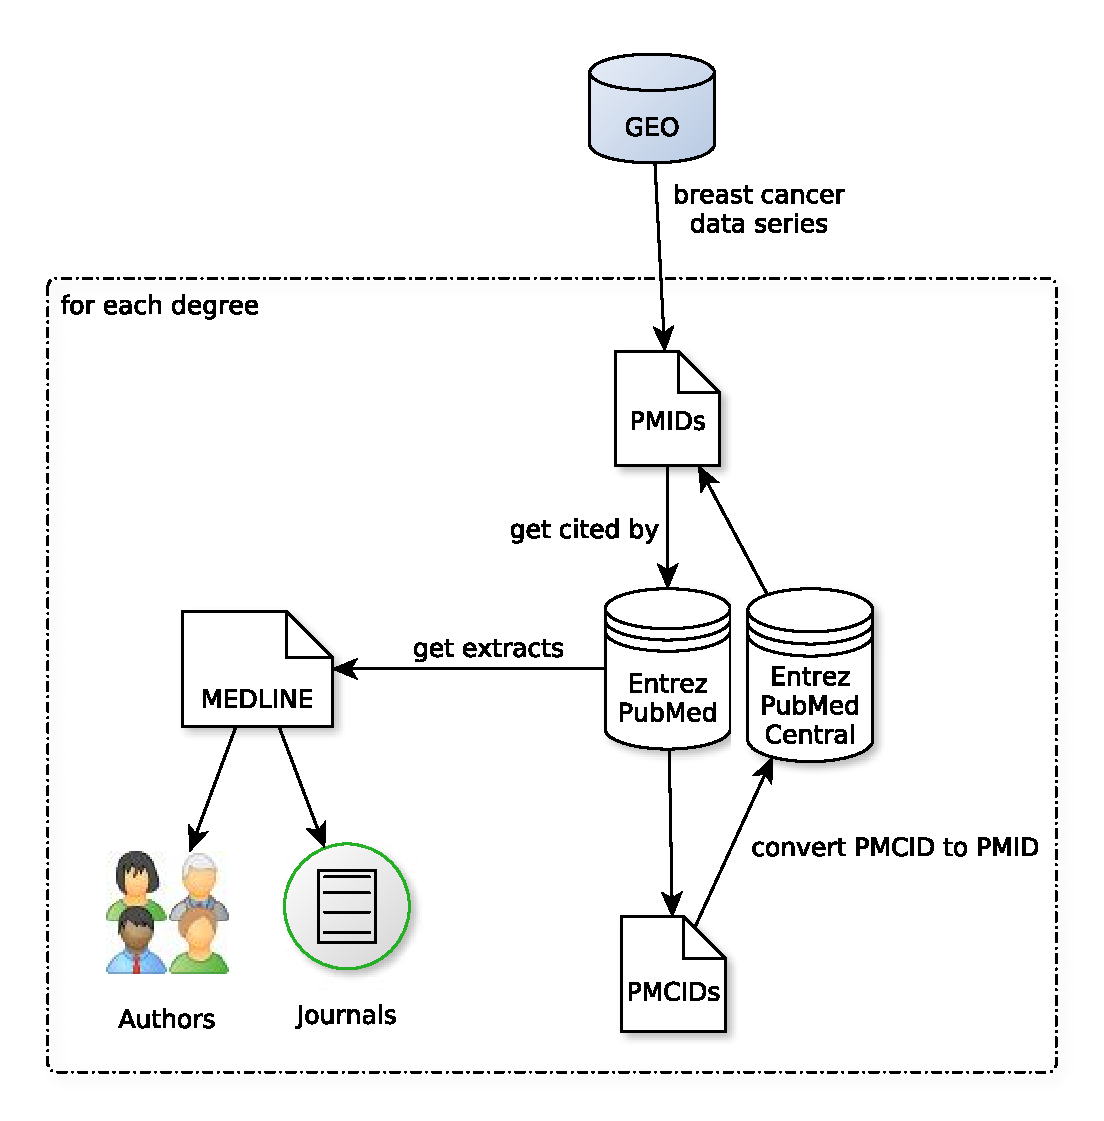
\includegraphics[width=\columnwidth]{ncbi_pipeline.eps}
    \caption{NCBI Query Pipeline}
    \label{fig:pipeline}
\end{figure}

From this, two preprocessing steps occur before arriving at the data used in our experiments. First, we only look at up to the first three authors plus the last author of a paper. Because of the interdisciplinary nature of biomedicine, many publications may consist of more than 20 authors or committees of people within an institution. The last author is used because it oftentimes corresponds to an adviser for the paper. Without a cap on four authors per paper, we expect the number of authors to increase following the paper size increase until the entire community is accounted. From this 57,332 author subset, we then delete 34,638 authors who had less than two papers in our corpus. Both of these choices are done to decrease the sparsity of our transition matrices and to obtain what we consider the important contributors for a paper. Second, we restrict the data to papers and authors attached to the top 100 journals, which include around 40\% of the publications and 50\% of the author subset. We make this restriction on journal number to increase the density of the tensors used in the multirank framework, where we have used journal as the relation connecting authors. After preprocessing, our data consists of 9,451 papers, associated with 9 datasets, written in 100 journals by 11,448 authors.

As a comparison, raw data used for the current DataRank prototype (queried in May 2014) contains around 2.7 million papers with 2,835,252 unique authors and 20,483 journals. From this, only 20,000 datasets are indexed, so the paper and author space is diminished significantly. We believe our experiments on a data size one hundredth of the size of unprocessed data used in DataRank is satisfactory for our exploratory methods to enhance the feature selection and ranking process of the existing prototype.

\paragraph{Data Statistics}
The following information gives a sense of the boundaries of our data to put into context the numbers shown in Result tables found in Section~\ref{sec:results}.

\begin{itemize}[noitemsep,nolistsep]
    \item Highest \# of publications: 28
    \item Authors with highest \# of publications: Perou, Charles M and Creighton, Chad J
    \item Mean number of paper per author: 2.13
    \item Median number of paper per author: 2
    \item Number of authors with no collaborators: 2,627
    \item Average number of collaborators for authors \footnote{authors with collaborations}: 3.58
    \item Highest number of collaborators: 44 for Creighton, Chad J
    \item Mean number of journals in which author is published: 1.83
    \item Mean number of papers per journal \footnote{of the top 100 journals}: 103.44
    \item Median number of papers per journal: 52.5
    \item Max/Min number of papers per journal: 1692 / 8
    \item Highest cited by count for PMID: 519
    \item Mean of cited by count for PMID: 13.04
    \item Median of cited by count for PMID: 5
\end{itemize}

\subsection{Corank}
Corank uses five parameters, but we set three parameters ($m,n,k = 1$) to simplify the implementation to only take into account two parameters: $\alpha = 0.1$ and $\lambda = 0.2$. The implicit parameters correspond to the number of intra-class and inter-class steps taken. With $k=1$, the inter-walk procedure in Algorithm~\ref{alg:inter} takes three substeps ($2k+1$). The authors of Corank suggest preventing large $k$ because it would eliminate the effects between authors and papers. The number of intra-class steps taken is governed by parameters $n,m$ for the citation and author network, respectively. Increasing these parameters means taking powers of $\tilde{A}^T$ and $\tilde{P}^T$ when updating $\mathbf{a}$ and $\mathbf{d}$ in Algorithm~\ref{alg:corank}. Changing these parameters did not greatly affect the top 20 authors or papers in the original corank experiments, so we set them to 1 for faster computation. As explained previously, $\alpha$ is like the dampening parameter used in PageRank that gives the probability a web surfer will continue clicking; the analogous value assumed in PageRank is 0.15. A larger $\alpha$ parameter would cause the transition matrices to be closer to uniform. $\lambda$ is the coupling factor for the random walks; the extremes of $\lambda=0,1$ correspond to taking either only intra-class walks or inter-class walks. 


\subsection{MultiRank}
Unlike Corank, there are no parameters needed --- only the definition of the tensor is required to implement Multirank. We define tensor $\mathcal{A}$ as author citations through journals, where authors act as objects and journals as relations. Thus the value of $a_{i_1,i_2,j_1}$ counts the instances where a paper written by author $i_1$ is cited by a paper written by author $i_2$ and both papers are published in journal $j_1$. Additionally, we restrict these counts to prevent self-citations such that $a_{i1,i1,j1} = 0$ for all authors and journal relations. With this representation, $\mathcal{A}$ is of size 11,448 by 11,448 by 100. Disregarding dangling nodes, $\mathcal{A}$ contains 15,021 non-zero entries, so the sparsity density is $1.146 \times 10^{-6} \%$. Our output is two ranking vectors $\mathbf{x}\in \mathbb{R}^{11448}$ and $\mathbf{y} \in \mathbb{R}^{100}$. The ranking for vector $\mathbf{x'}$ is disregarded because our data is only generated from a `cited by' relationship, rather than a `cites' relationship, though both vectors are used in the iterative algorithm. 

\paragraph{Sparsity Issue}
With such a highly sparse tensor, many of the tensor entries needed to be set as dangling nodes with the probability $\frac{1}{d}$. Filling in these entries resulted in a huge tensor, so an alternative method of computing the probabilities in equations~\ref{eq:vec_x} and~\ref{eq:vec_y} is required to deal with the dangling node issue. This is done by using linear indices, saving the the indices of non-dangling nodes and dangling nodes, and computing each entry of the stationary probability as a non-dangling portion plus the dangling portion. Since the dangling portion is constant, it can be precomputed and reused. 

We show the calculation for $\mathbf{x}$ as an example and make use of MATLAB's conversion of matrix subscripts to linear indices. For a particular $i_1$,

\begin{align*}
    x_i &= \sum_{i_2,j_1} \hat{O}_{i,i_2,j_1} M_{i_2,j_1} \\
                &= \textsc{sub2ind}(\hat{O}_{i,:,:})^T \textsc{sub2ind}(M) \\
                &= \textsc{sub2ind}(O_{i,idx})^T \textsc{sub2ind}(M(idx)) + \frac{1}{m} \sum_{i_2,j} M(dng) 
\end{align*}

where $M=\mathbf{xy^T}$ and $$
\hat{O}_{i,i_2,j_1} =
\begin{cases}
O_{i,i_2,j_1}, & i_2,j \in \text{idx} \\
\frac{1}{m}, & i_2,j \in \text{dng}
\end{cases} $$


\section{Results and Discussion}
\label{sec:results}
All experiments used an epsilon value of 1e-10 as the difference between iterative computations of the probability distributions. Unfortunately, the ranking results are inherently difficult to quantify, especially without first defining an appropriate loss/cost function that captures exactly what and how one would measure `importance'. Once these results are scaled up to integrate the 20,000 datasets indexed in the DataRank prototype, users can be brought in for testing. However, before that occurs we conduct a solely qualitative evaluation, like that used by Corank and Multirank. We differ in that we try to examine quantities captured by the network structure, while other evaluations rely on agreement between `expert judges' that numerically assess authors based on knowledge of their research domain community.

\paragraph{Paper Ranking}\footnote{Italicized PMID indicate original paper of data series}
Individual ranking of papers took 151 iterations to converge in 12.45 seconds. As can be seen from Table~\ref{tab:paper_rank}, there is little variability between the top 15 papers when ranked individually and coranked. The six original papers which were cited more than hundreds of times appear in the top nine rankings. It is not entirely clear why PMID 17069663 and 16417655 are so highly ranked because they have low cited by counts, but it should be noted that they do cite the top ranked original paper.

    \begin{table}[h]
    \resizebox{\columnwidth}{!}{
    \begin{tabular}{|c|cc|cc|}
    \hline
    \textbf{Ranking} & \textbf{PMID (Indiv.)} & \textbf{\# Cited By} & \textbf{PMID (Corank)} & \textbf{\# Cited By} \\ \hline
    1 & \textit{12297621} & 212 & \textit{12297621} & 212 \\
    2 & \textit{16273092} & 418 & \textit{16273092} & 418 \\
    3 & \textit{15193263} & 129 & \textit{15193263} & 129 \\
    4 & \textit{16141321} & 337 & \textit{16141321} & 337 \\
    5 & \textit{16478745} & 342 & \textit{16478745} & 342 \\
    6 & 17069663 & 12 & 17157791 & 519 \\
    7 & 17157791 & 519 & 16643655 & 254 \\
    8 & 16643655 & 254 & \textit{16280042} & 203 \\
    9 & \textit{16280042} & 203 & 15034139 & 54 \\
    10 & 15034139 & 54 & 18948947 & 284 \\
    11 & 18948947 & 284 & 18443585 & 297 \\
    12 & 16585533 & 82 & 16585533 & 82 \\
    13 & 18443585 & 297 & 17493263 & 210 \\
    14 & 16417655 & 20 & 16417655 & 20 \\
    15 & 17493263 & 210 & 17069663 & 12 \\ \hline
    \end{tabular}}
    \caption{Paper Ranking: Individual vs. Corank}
    \label{tab:paper_rank}
    \end{table}

Table~\ref{tab:paper_ranking_analysis} displays the rankings for the nine original papers that appeared in the top 100 journals, and shows that there is little difference between individual and coranking. As an aside, we include the number of samples for each dataset. We also display the cumulative number of publications within our corpus by the authors of the dataset. We admit it is difficult to evaluate the output of the paper rankings. Ranking papers more effectly would require more processing, perhaps first running a topic model and then ranking within a research area. Fortunately, we are more interested in the results of the author ranking for augmenting the DataRank prototype.

    \begin{table}[h]
    \resizebox{\columnwidth}{!}{
    \begin{tabular}{c|c|ccc|}
    \cline{2-5}
    {\color[HTML]{9B9B9B} {\bf \# Data Samples}} & {\bf Original PMID} & {\bf Indiv. Rank} & {\bf Corank} & {\bf Cited By} \\ \cline{2-5} 
    {\color[HTML]{9B9B9B} 100} & 12297621 & 1 & 1 & 212 \\
    {\color[HTML]{9B9B9B} 158} & 16273092 & 2 & 2 & 418 \\
    {\color[HTML]{9B9B9B} 60} & 15193263 & 3 & 3 & 129 \\
    {\color[HTML]{9B9B9B} 502} & 16141321 & 4 & 4 & 337 \\
    {\color[HTML]{9B9B9B} 189} & 16478745 & 5 & 5 & 342 \\
    {\color[HTML]{9B9B9B} 318} & 16280042 & 9 & 8 & 203 \\
    {\color[HTML]{9B9B9B} 126} & 16626501 & 20 & 20 & 36 \\
    {\color[HTML]{9B9B9B} 180} & 16505412 & 25 & 26 & 37 \\
    {\color[HTML]{9B9B9B} 17} & 16849584 & 44 & 51 & 42 \\ \cline{2-5} 
    \end{tabular}}
    \caption{Paper Ranking Analysis}
    \label{tab:paper_ranking_analysis}
    \end{table}

    % \begin{table}[h]
    % \resizebox{\columnwidth}{!}{
    % \begin{tabular}{|c|cccc|}
    % \hline
    % \textbf{Original PMID} & \textbf{Individual Rank} & \textbf{Corank} & \textbf{\# Cited By} & \textbf{\# Papers for Authors} \\ \hline
    % 12297621 & 1 & 1 & 212 & 55 \\
    % 16273092 & 2 & 2 & 418 & 31 \\
    % 15193263 & 3 & 3 & 129 & 14 \\
    % 16141321 & 4 & 4 & 337 & 13 \\
    % 16478745 & 5 & 5 & 342 & 31 \\
    % 16280042 & 9 & 8 & 203 & 11 \\
    % 16626501 & 20 & 20 & 36 & 14 \\
    % 16505412 & 25 & 26 & 37 & 15 \\
    % 16849584 & 44 & 51 & 42 & 20 \\ \hline
    % \end{tabular}}
    % \caption{Paper Ranking Analysis}
    % \label{tab:paper_ranking_analysis}
    % \end{table}


\paragraph{Individual Author Ranking} \footnote{Italicized names indicate authors of original paper of data series}
Individual author ranking took 32 iterations to converge in 15.66 sec. From Table~\ref{tab:author_indiv}, one can observe the general trend that authors with many collaborations are highly individually ranked. This trend is not a surprise because of how individual ranking works --- by using the structure of the collaboration network. An author with more links and stronger links simply has higher probability of being visited in a random walk. As an example, we attempt to explain why Nevins (rank 8) ranks higher than Pollack (rank 9). Both have the same number of publications; Nevins has fewer coauthors but his coauthor links are stronger with a sum of 48 links (vs. a sum of 45 links for Pollack). Individual ranking only takes place on the author graph, so the number of papers should not affect its outcome. However, having many publications and having many coauthors usually go hand in hand. Only three of the top 15 authors, who also happen to be highly coranked, are associated with the original papers. 

    \begin{table}[h]
    \resizebox{\columnwidth}{!}{
    \begin{tabular}{|c|ccccc|}
    \hline
    \textbf{Indiv. Ranking} & \textbf{Author} & \textbf{\# Coauthors} & \textbf{\# Papers} & \textbf{Rank in Corank} & \textbf{Rank in Multirank} \\ \hline
    1 & Creighton, Chad J & 44 & 28 & 39 & 66 \\
    2 & \textit{Perou, Charles M} & 43 & 28 & 1 & 3 \\
    3 & Zhang, Wei & 22 & 18 & 292 & 500+ \\
    4 & Pusztai, Lajos & 36 & 21 & 63 & 318 \\
    5 & Teschendorff, Andrew E & 30 & 21 & 43 & 7 \\
    6 & Haibe-Kains, Benjamin & 33 & 22 & 34 & 500+ \\
    7 & Massague, Joan & 21 & 19 & 10 & 74 \\
    8 & \textit{Nevins, Joseph R} & 24 & 19 & 5 & 198 \\
    9 & \textit{Pollack, Jonathan R} & 25 & 19 & 2 & 2 \\
    10 & Chinnaiyan, Arul M & 23 & 20 & 128 & 500+ \\
    11 & Arteaga, Carlos L & 23 & 21 & 211 & 500+ \\
    12 & Katzenellenbogen, Benita S & 29 & 16 & 82 & 16 \\
    13 & Liu, Edison T & 23 & 13 & 31 & 103 \\
    14 & Caldas, Carlos & 31 & 18 & 47 & 23 \\
    15 & Weinberg, Robert A & 18 & 17 & 21 & 98 \\ \hline
    \end{tabular}}
    \caption{Top Authors by Individual Ranking}
    \label{tab:author_indiv}
    \end{table}


\paragraph{Author Corank}
Coranking (both papers and authors) took 74 iterations to converge in 11.58 sec. Already we see an improvement to individual ranking with eleven of the top fifteen being authors associated with the original papers. We expect authors with many publications and many coauthors to be ranked highly, which is generally the case, but there are some authors with few papers that appear highly ranked. We suspect this is because they are mostly original authors who are coauthored with an author of high rank or connected to papers with a high number of citations. For example, authors Ma, Yao, Sorlie (ranked 6, 13, 14, respectively) all have less than 5 publications and less than or equal to 10 coauthors but they are original authors and strongly connected to Perou, Pollack, Brown, and Nevins (ranked 1, 2, 3, 5, respectively). Authors Bergh and Miller (ranked 9 and 12) also have few paper and coauthor counts, but they are the authors of highly individually ranked PMID 161413321 (337 citations). Seventh ranked You is not an original author but he has coauthored multiple times with highly ranked Nevins and Yao. Tenth ranked Massague is also not an original author, but her total citation count of 466 is almost double than what would be expected based on her publication number and the mean PMID cited by count of 13. 

    \begin{table}[h]
    \resizebox{\columnwidth}{!}{
    \begin{tabular}{|c|ccccc|}
    \hline
    \textbf{Corank} & \textbf{Author} & \textbf{\# Papers} & \textbf{\# Coauthors} & \textbf{Rank Individually} & \textbf{Rank in Multirank} \\ \hline
    1 & \textit{Perou, Charles M} & 28 & 43 & 2 & 3 \\
    2 & \textit{Pollack, Jonathan R} & 19 & 25 & 9 & 2 \\
    3 & \textit{Brown, Patrick O} & 6 & 8 & 381 & 100 \\
    4 & \textit{Sgroi, Dennis C} & 11 & 25 & 29 & 30 \\
    5 & \textit{Nevins, Joseph R} & 19 & 24 & 8 & 198 \\
    6 & \textit{Ma, Xiao-Jun} & 4 & 6 & 413 & 41 \\
    7 & You, Lingchong & 8 & 5 & 119 & 500+ \\
    8 & \textit{Chang, Jeffrey T} & 12 & 19 & 51 & 316 \\
    9 & \textit{Bergh, Jonas} & 4 & 8 & 917 & 1 \\
    10 & Massague, Joan & 19 & 21 & 7 & 74 \\
    11 & Parker, Joel S & 14 & 26 & 53 & 6 \\
    12 & \textit{Miller, Lance D} & 7 & 14 & 190 & 12 \\
    13 & \textit{Yao, Guang} & 5 & 7 & 1229 & 500+ \\
    14 & \textit{Sorlie, Therese} & 5 & 10 & 1474 & 43 \\
    15 & Lam, Wan L & 22 & 21 & 17 & 58 \\ \hline
    \end{tabular}}
    \caption{Top Authors by Corank}
    \label{tab:author_corank}
    \end{table}



\paragraph{Multirank}
Multiranking authors with journal relations took 21 iterations to converge in 78.2 sec. Eleven of the top fifteen are original authors, but they are not the same eleven that appear for corank; however, there is an overlap of five authors, four of which are original authors. Interestingly, the bottom half of Table~\ref{tab:multi} have few papers, and are very lowly ranked individually, but the papers they've published are highly cited, published in the top journals, and thus they make up a strong portion of the overall network. 

Chin (ranked 10) and Bocanegra (ranked 13) seem like outliers as they are neither original authors nor have many papers and coauthors. However, one of the two papers authored by Chin has a 519 cited by count, which makes it the top cited paper. Bocanegra coauthored both papers with 2nd ranked Pollack, and her papers cite three of the original papers.

    \begin{table}[h]
    \resizebox{\columnwidth}{!}{
    \begin{tabular}{|c|ccccc|}
    \hline
    \textbf{Multirank} & \textbf{Author} & \textbf{\# Papers} & \textbf{\# Coauthors} & \textbf{Rank in Corank} & \textbf{Rank Individually} \\ \hline
    1 & \textit{Bergh, Jonas} & 4 & 8 & 9 & 917 \\
    2 & \textit{Pollack, Jonathan R} & 19 & 25 & 2 & 9 \\
    3 & \textit{Perou, Charles M} & 28 & 43 & 1 & 2 \\
    4 & \textit{Sotiriou, Christos} & 15 & 25 & 16 & 48 \\
    5 & \textit{Pawitan, Yudi} & 8 & 17 & 19 & 84 \\
    6 & Parker, Joel S & 14 & 26 & 11 & 53 \\
    7 & Teschendorff, Andrew E & 21 & 30 & 43 & 5 \\
    8 & \textit{Delorenzi, Mauro} & 8 & 11 & 23 & 195 \\
    9 & \textit{Wirapati, Pratyaksha} & 5 & 12 & 50 & 1266 \\
    10 & Chin, Koei & 2 & 4 & 70 & 7421 \\
    11 & \textit{Bjohle, Judith} & 1 & 2 & 79 & 9435 \\
    12 & \textit{Miller, Lance D} & 7 & 14 & 12 & 190 \\
    13 & Bocanegra, Melanie & 2 & 5 & 269 & 8421 \\
    14 & \textit{George, Joshy} & 4 & 7 & 34 & 2281 \\
    15 & \textit{Smeds, Johanna} & 1 & 3 & 80 & 10788 \\ \hline
    \end{tabular}}
    \caption{Top Authors by Multirank}
    \label{tab:multi}
    \end{table}

Ranking of the top ten journals seen in Table~\ref{tab:journal} suggest that the general trend is to rank by number of papers published within a journal. Journals with many publications inherently leads to more authors, and probably with authors of higher influence within the network. The lower ranking for journal 5 and 6 which both published a paper connected to an original dataset may suggest that the original paper does not have a great influence on the journal rank. This may be because those original papers are not as highly cited as other papers. Regardless, we note that the original nine papers appear in the top 27 journals.

    \begin{table}[h]
    \resizebox{\columnwidth}{!}{
    \begin{tabular}{|c|lcc|}
    \hline
     & \multicolumn{1}{c}{{\bf Journal}} & {\bf \# Papers} & {\bf \# Originals} \\ \hline
    {\bf 1} & PloS one & 1692 & --- \\
    {\bf 2} & Breast cancer research : BCR & 483 & 2 \\
    {\bf 3} & Proceedings of the National Academy of Sciences of the USA & 419 & 2 \\
    {\bf 4} & BMC bioinformatics & 369 & --- \\
    {\bf 5} & Cancer research & 422 & 1 \\
    {\bf 6} & Cancer cell & 136 & 1 \\
    {\bf 7} & Bioinformatics (Oxford, England) & 174 & --- \\
    {\bf 8} & BMC genomics & 289 & --- \\
    {\bf 9} & Genome research & 130 & --- \\
    {\bf 10} & The Journal of clinical investigation & 156 & --- \\ \hline
    \end{tabular}}
    \caption{Top Multiranked Journals}
    \label{tab:journal}
    \end{table}


    \begin{figure}[t!]
        \centering
        \subfigure[Author Multirank]{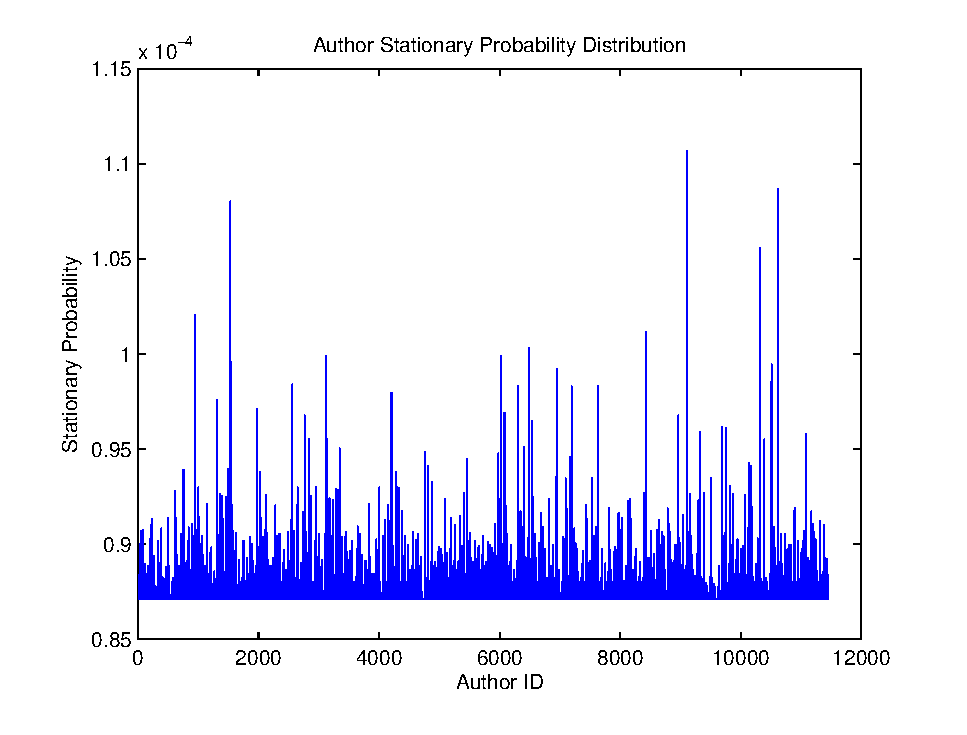
\includegraphics[width=\columnwidth]{author_dist.eps}}
        \subfigure[Journal Multirank]{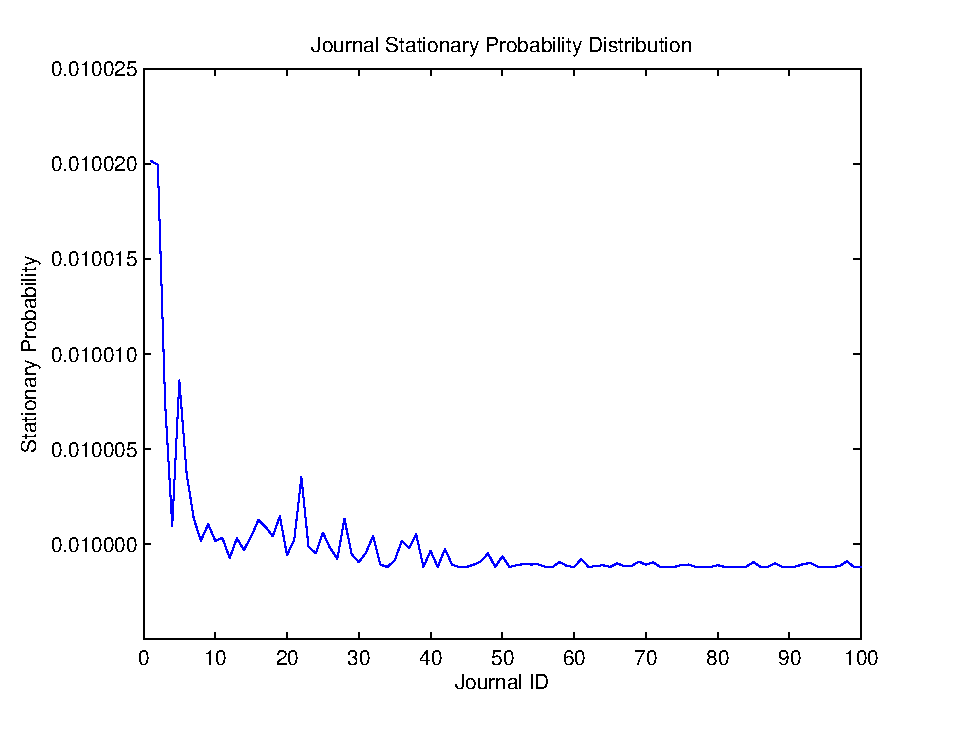
\includegraphics[width=\columnwidth]{journal_dist.eps}}
        \caption{Multirank Stationary Probability Vectors}
        \label{fig:stable}
    \end{figure}

    \begin{figure}[h]
        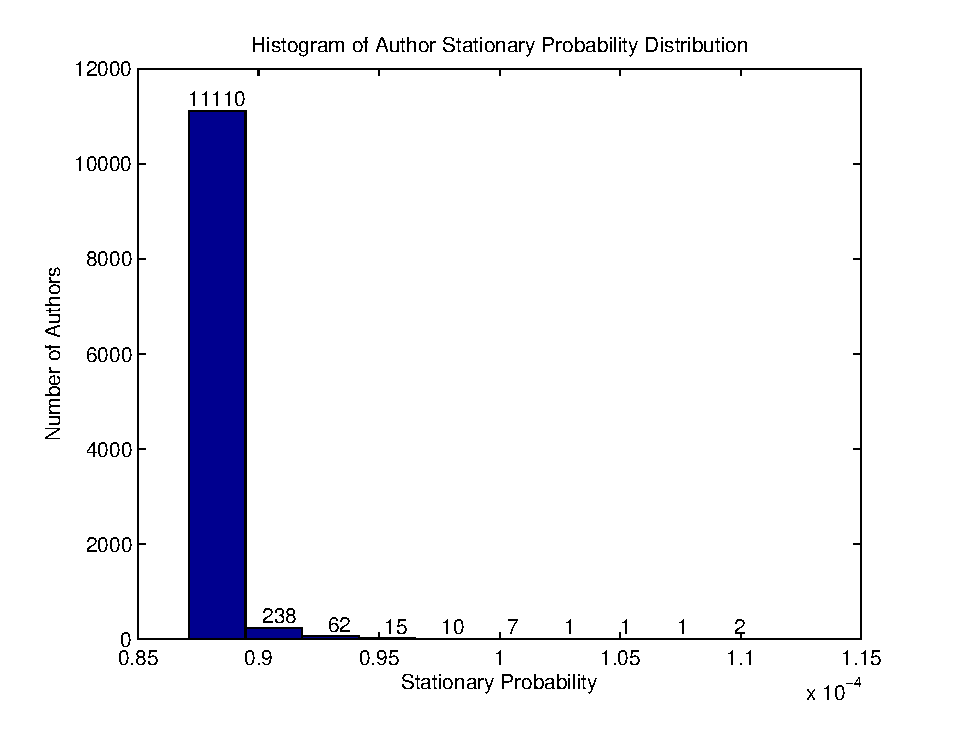
\includegraphics[width=\columnwidth]{author_hist.eps}
        \caption{Histogram of Author Distribution}
        \label{fig:auth_hist}
    \end{figure}

Figure~\ref{fig:stable} shows the plot of the stable probability distribution for journals and authors. From this we can see that there is a clear different in multirank values for authors, but the journal multirank is fairly uniform with a very narrow range of probability values (almost equal to the dangling node probability of $\frac{1}{n=100}$). This hints at two things: firstly, we can take a histogram plot of the author distribution to get a sense of the size of author set to focus on. As seen in Figure~\ref{fig:auth_hist}, only about 100 authors have some significant rank and probably make up a subnetwork of interest. Secondly, the journal relation turns out to be quite insignificant, and thus merely adds complexity to the model. Without the journal relation, Multirank essentially becomes something close to PageRank for authors; but even with journal ranks, which seems nondistinguishing, Multirank has somehow captured the importance of original authorship. We propose some alternative experiments using different relations to explore in the Future Work subsection.



\subsection{Connecting Ranking to Datasets}
In order to obtain conditional probabilities between authors and datasets, we first count the occurences of authors with journals in our underlying data and normalize this to create a joint probability $Pr(Author,Journal)$. This joint can be divided by the learned multiranking for authors $\mathbf{x} = Pr(Author)$ and $\mathbf{y}=Pr(Journal)$ to get conditional probabilities which can be represented as a matrix $M_{A,J}$ of dimension $|A|\times|J|$. To get the connection between author and dataset, we first calculate a linear weighting for datasets. This is calculated for each journal by counting how many times a dataset is connected to the papers published in that journal. $Pr(D=d_1|J=`Plos one')$ is the weighting of dataset 1 for all the datasets connected to papers published in Plos one. A more fine grained weighting would also take into account if the citation to the dataset was a direct citation or required a longer path which requires another run of querying NCBI. Then by multiplying matrix $M_{A,J}$ by the journal-dataset weightings, we obtain a matrix of size $|A|\times|D|$. Each row essentially describes the weighting of datasets and thus a dataset rank for a given author. 

The top three recommended datasets for the top five Multiranked authors is as follows:
    \begin{table}[h]
    \resizebox{\columnwidth}{!}{
    \begin{tabular}{|c|c|ccc|}
    \hline
    \textbf{Original} & \textbf{Author} & \textbf{Rec 1} & \textbf{Rec 2} & \textbf{Rec 3} \\ \hline
    GSE3494 & Bergh, Jonas & GSE2607 & GSE3453 & GSE1378 \\
    GSE3281 & Pollack, Jonathan R & GSE1378 & \textit{GSE3281} & GSE3143 \\
    GSE3281 & Perou, Charles M & GSE1378 & GSE3453 & GSE2990 \\
    GSE2990 & Sotiriou, Christos & GSE3453 & \textit{GSE2990} & GSE1456 \\
    GSE1456 & Pawitan, Yudi & GSE3453 & GSE2990 & \textit{GSE1456} \\ \hline
    \end{tabular}}
    \caption{Dataset Recommendation for Top 5 Multiranked Authors}
    \label{tab:rec}
    \end{table}

\section{Discussion}
It is difficult to determine whether Corank or Multirank is a better qualitative fit for our needs as both return sensible author rankings. However, we prefer to explore Multirank further because it is more easily extendable and leads to more hypotheses to test. While we have only explored one connection of author citations through journals, the framework allows for higher order tensor constructions that could capture more relationships and object types. Another reason is because Multirank has no parameters and thus no tuning or justification for parameters. With only three graphs, Corank already has five parameters (three with our simplified approach). Altering it to work with more networks would exponentially increase the number of parameters: just adding an additional network to the existing framework would require another intra-walk parameter, two inter-walk parameters, two coupling parameters, and potentially another dampening factor.

\subsection{Future Work}
An obvious extension is to combine ranking with clustering by examining the frameworks used in~\cite{sun2009rankclus} and~\cite{varadharajalu2011author}. However, our existing experiements could also be improved by defining different relations. Finally, this work needs to be incorporated into the existing prototype and tested with users. With user testing, we can actually begin to quantify the usefulness of these recommendations. Incorporating this requires scaling the frameworks to include the 20,000 datasets currently used in DataRank. Obtaining this data requires first crawling the GEO repository for the original PMID associated with the dataset, then making the relevant NCBI queries to create the underlying data. It is no surprise that the result of this would be sparse. This sparsity is another reason why we favor Multirank over Corank for the next step of the experimentation as the representation and computation of such sparsity can be more easily implemented with Multirank.

\paragraph{Alternative to Multirank Independence Assumption}
\label{para:alternative}
As mentioned previously, in calculating Multirank we assume independence such that the joint probability of $Pr(X_{t-1}=i_2,Y_t=j_1) = Pr(X_{t-1}=i_2)Pr(Y_t=j_1)$. Here we propose an alternative to this assumption by first assuming independence, then separately learning this by calculating $$Pr(X_{t-1}=i_2,Y_t=j_1) = Pr(X_{t-1}=i_2|Y_t=j_1)Pr(Y_t=j_1)$$ Extra notation is needed:
\begin{table}[h]
\begin{tabular}{l}
$\mathcal{O} = Pr(X_1|X_2,Y)$ \\
$\mathcal{R}=Pr(Y|X_1,X_2)$ \\
$\mathcal{Q}=Pr(X_2|X_1,Y)$ \\
$\mathbf{U} = Pr(X_2|Y) = \sum_{i_1} Pr(X_2|X_1,Y) Pr(X_1|Y) = \sum_{i_1} \mathcal{Q}\mathbf{V}$ \\
$\mathbf{V} = Pr(X_1|Y) = \sum_{i_2} Pr(X_1|X_2,Y) Pr(X_2|Y) =\sum_{i_2} \mathcal{O}\mathbf{U}$ \\
$\mathbf{Z} = Pr(X_2|X_1) = \sum_j Pr(X_2|X_1,Y) Pr(Y|X_1) =\sum_j \mathcal{Q}\mathbf{W}$ \\
$\mathbf{W} = Pr(Y|X_1) = \sum_{i_2} Pr(Y|X_1,X_2) Pr(X_2|X_1) =\sum_{i_2} \mathcal{R}\mathbf{Z}$
\end{tabular}
\end{table}

First, we run our existing multirank algorithm to get some initial values for $\mathbf{x_1,x_2,y}$. These can be used as the initial values to calculate $\mathbf{U,V,W,Z}$. Lastly, $\mathbf{x_1,y}$ is calculated with by
\begin{align*}
    \mathbf{x_1} &= \sum_{i_2}\mathcal{O}\mathbf{Uy} = \mathbf{Vy} \\
    \mathbf{y} &= \sum_{i_2}\mathcal{R}\mathbf{Zx_1} = \mathbf{Wx_1}
\end{align*}
These last two subprocesses would be repeated until convergence of $\mathbf{x_1,y}$.

\paragraph{Multirank Relations to Explore}
Some other relations to explore to get more variability in relation multiranking include using MeSH terms or datasets as relation instead of journal. By looking at citation counts for top multiranked authors to top datasets, one could potentially locate clusters to see if particular authors act more as dataset or methodology contributors or dataset curators. Other connections to explore would be author collaborations rather than author citations. The results of these could be compared to see which journals (or datasets or MeSH terms) may lead to more collaboration versus citations.

Additionally, for every dataset, one could create an author by author collaboration matrix to get conditional proability of authors given dataset and compare this result with our conditional probability tables. While this would not be difficult to implement, it would require different NCBI querying than what was already completed for these experiments in order to generate the underlying experimental data. 

\section{Conclusions}

In this project, we investigated heterogeneous citation and coauthorship networks connected to nine breast cancer data series from the Gene Expression Omnibus repository and compared three ranking algorithms (baseline individual network ranking, Corank, and Multirank). Based on our limited preliminary study, we showed that the Multirank approach based on a tensor representation holds great promise to the DataRank project, but multi-faceted data collection and fine-grained annotations are still necessary to make the best use of this technique for personalized information retrieval.


% \clearpage
\bibliographystyle{abbrv}
\bibliography{sources}  
\balancecolumns

\end{document}